\subsection{Independent Change}

\begin{figure}[htbp]
\centerline{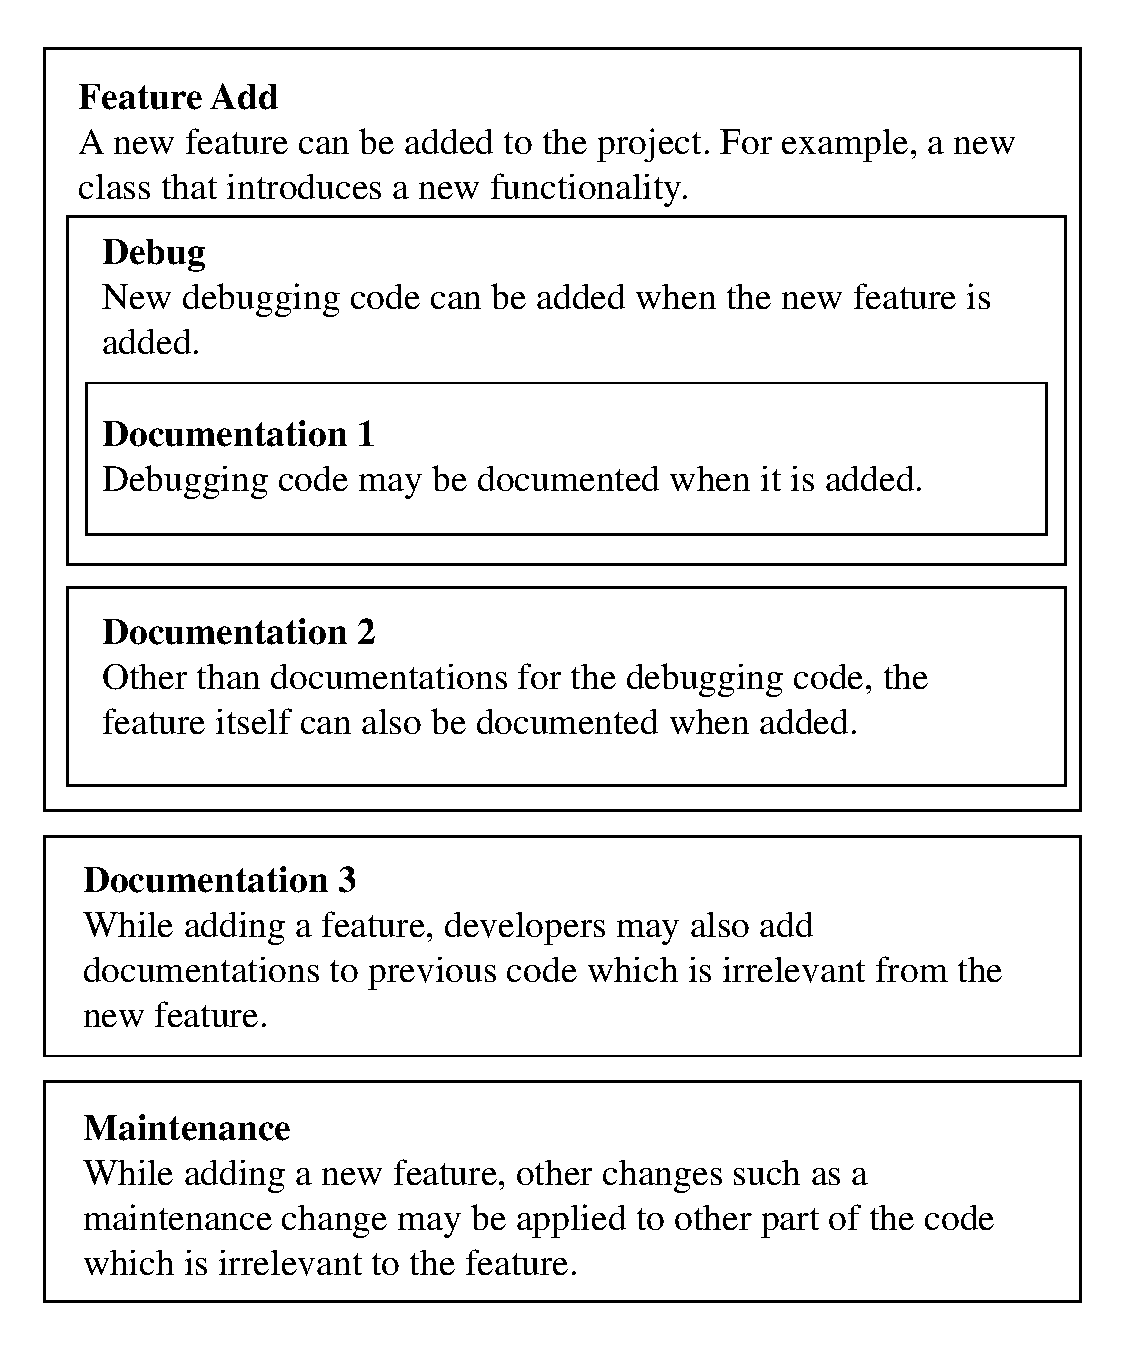
\includegraphics[scale=0.5]{figures/independent_change.pdf}}
\caption{Explanation For Independent Change}
\label{fig:Relationship}
\end{figure}

To improve our tagging, we first note that the original change type definitions overlap. For example, a documentation change may occur as part of a feature add commit. This increases tagging ambiguity and complexity, which we solve by introducing the concept of an \textit{independent change}.

We call a change an \textit{independent change} when it is not a part of other changes.
Fig. \ref{fig:Relationship} explains this concept. It illustrates a commit with multiple changes, in which a new feature contains three sub-changes.
Each block represents a code change. 
In the figure, a new feature change contains debugging code, documentation 1 for the functionality of the feature, documentation 2 for the debugging code, an irrelevant documentation 3, and an irrelevant maintenance change. 
In this case, the debugging code and documentation 1 and 2 are sub-changes to the new feature. 
As a result, we only assign a ``Feature Add'' tag to the new feature instead of assigning tags to all sub-changes. 
As documentation 3 and maintenance are both unrelated to the new feature, they will be assigned Documentation and Maintenance tags.
The new feature, documentation 3, and maintenance groups are independent changes, with the associated three independent tags forming a label the commit. 
With the introduction of independent change types, we reduce the ambiguity in the initial taxonomy which results in fewer cross-validation errors and improved tagging efficiency.
